% Options for packages loaded elsewhere
\PassOptionsToPackage{unicode}{hyperref}
\PassOptionsToPackage{hyphens}{url}
\documentclass[
  ignorenonframetext,
]{beamer}
\newif\ifbibliography
\usepackage{pgfpages}
\setbeamertemplate{caption}[numbered]
\setbeamertemplate{caption label separator}{: }
\setbeamercolor{caption name}{fg=normal text.fg}
\beamertemplatenavigationsymbolsempty
% remove section numbering
\setbeamertemplate{part page}{
  \centering
  \begin{beamercolorbox}[sep=16pt,center]{part title}
    \usebeamerfont{part title}\insertpart\par
  \end{beamercolorbox}
}
\setbeamertemplate{section page}{
  \centering
  \begin{beamercolorbox}[sep=12pt,center]{section title}
    \usebeamerfont{section title}\insertsection\par
  \end{beamercolorbox}
}
\setbeamertemplate{subsection page}{
  \centering
  \begin{beamercolorbox}[sep=8pt,center]{subsection title}
    \usebeamerfont{subsection title}\insertsubsection\par
  \end{beamercolorbox}
}
% Prevent slide breaks in the middle of a paragraph
\widowpenalties 1 10000
\raggedbottom
\AtBeginPart{
  \frame{\partpage}
}
\AtBeginSection{
  \ifbibliography
  \else
    \frame{\sectionpage}
  \fi
}
\AtBeginSubsection{
  \frame{\subsectionpage}
}
\usepackage{iftex}
\ifPDFTeX
  \usepackage[T1]{fontenc}
  \usepackage[utf8]{inputenc}
  \usepackage{textcomp} % provide euro and other symbols
\else % if luatex or xetex
  \usepackage{unicode-math} % this also loads fontspec
  \defaultfontfeatures{Scale=MatchLowercase}
  \defaultfontfeatures[\rmfamily]{Ligatures=TeX,Scale=1}
\fi
\usepackage{lmodern}
\ifPDFTeX\else
  % xetex/luatex font selection
\fi
% Use upquote if available, for straight quotes in verbatim environments
\IfFileExists{upquote.sty}{\usepackage{upquote}}{}
\IfFileExists{microtype.sty}{% use microtype if available
  \usepackage[]{microtype}
  \UseMicrotypeSet[protrusion]{basicmath} % disable protrusion for tt fonts
}{}
\makeatletter
\@ifundefined{KOMAClassName}{% if non-KOMA class
  \IfFileExists{parskip.sty}{%
    \usepackage{parskip}
  }{% else
    \setlength{\parindent}{0pt}
    \setlength{\parskip}{6pt plus 2pt minus 1pt}}
}{% if KOMA class
  \KOMAoptions{parskip=half}}
\makeatother
\usepackage{graphicx}
\makeatletter
\newsavebox\pandoc@box
\newcommand*\pandocbounded[1]{% scales image to fit in text height/width
  \sbox\pandoc@box{#1}%
  \Gscale@div\@tempa{\textheight}{\dimexpr\ht\pandoc@box+\dp\pandoc@box\relax}%
  \Gscale@div\@tempb{\linewidth}{\wd\pandoc@box}%
  \ifdim\@tempb\p@<\@tempa\p@\let\@tempa\@tempb\fi% select the smaller of both
  \ifdim\@tempa\p@<\p@\scalebox{\@tempa}{\usebox\pandoc@box}%
  \else\usebox{\pandoc@box}%
  \fi%
}
% Set default figure placement to htbp
\def\fps@figure{htbp}
\makeatother
\setlength{\emergencystretch}{3em} % prevent overfull lines
\providecommand{\tightlist}{%
  \setlength{\itemsep}{0pt}\setlength{\parskip}{0pt}}
\usepackage{bookmark}
\IfFileExists{xurl.sty}{\usepackage{xurl}}{} % add URL line breaks if available
\urlstyle{same}
\hypersetup{
  hidelinks,
  pdfcreator={LaTeX via pandoc}}

\author{\texorpdfstring{}{}}
\date{}

\begin{document}

\section{Discourse Circuits: Entity Persistence and
DisCoCirc}\label{sec:discocirc}

\subsection{The Compact Closure Axiom and Diagrammatic Complexity
Metrics}\label{the-compact-closure-axiom-and-diagrammatic-complexity-metrics}

\begin{frame}[fragile]{The Snake Equation (Zigzag Identity)}
\protect\phantomsection\label{the-snake-equation-zigzag-identity}
The algebraic engine of DisCoCat is the \textbf{compact closure} of the
pregroup category: for every type \(n\), the adjunction maps
\(\eta_n: 1 \to n \otimes n^r\) (cap) and
\(\varepsilon_n: n^r \otimes n \to 1\) (cup) satisfy the \textbf{snake
equation} (also called the zigzag identity):

\[(\varepsilon_n \otimes 1_n) \circ (1_n \otimes \eta_n) = 1_n \]
\{\#eq:eq-4-3\}

In string-diagrammatic terms, a cup composed with a cap on adjacent
wires ``straightens out'' into an identity wire---a zigzag that cancels
into a straight line. This axiom is not merely a formal curiosity: it is
the \emph{engine} that makes pregroup type reductions work. Every
grammatical contraction (noun canceling with verb argument) is an
instance of the cup map \(\varepsilon\), and every expansion
(introducing an adjoint pair) is an instance of the cap map \(\eta\).
The snake equation guarantees that these contractions and expansions are
well-behaved---they can be freely inserted and removed without changing
the meaning of the derivation.

The cognitive significance of the snake equation is that it provides a
\emph{visual proof} of coherence: an agent inspecting a string diagram
can verify that the derivation is well-formed by checking that all
zigzags cancel---a spatial operation that requires no algebraic
computation. This is precisely Shimojima's
{[}-@shimojima1996reasoning{]} ``free ride'' in its purest form.

\begin{figure}
\centering
\pandocbounded{\includegraphics[keepaspectratio,alt={The compact closure axiom ({[}@eq:eq-4-3{]}) rendered by DisCoPy as the snake equation: the left panel shows the zigzag diagram (\textbackslash varepsilon\_n \textbackslash otimes 1\_n) \textbackslash circ (1\_n \textbackslash otimes \textbackslash eta\_n) where a Cup contraction \textbackslash varepsilon composed with a Cap expansion \textbackslash eta on adjacent wires forms a snake; the right panel shows the identity wire 1\_n it equals. This identity---verified computationally via diagram.normal\_form() == Id(Ty(\textquotesingle x\textquotesingle))---is the algebraic engine powering every pregroup type reduction in : each grammatical contraction (noun canceling with verb argument) is an instance of \textbackslash varepsilon, and the snake equation guarantees that insertions and removals of cup-cap pairs leave derivations invariant.}]{output/figures/discopy_snake.png}}
\caption{The compact closure axiom ({[}@eq:eq-4-3{]}) rendered by
DisCoPy as the snake equation: the left panel shows the zigzag diagram
\((\varepsilon_n \otimes 1_n) \circ (1_n \otimes \eta_n)\) where a Cup
contraction \(\varepsilon\) composed with a Cap expansion \(\eta\) on
adjacent wires forms a snake; the right panel shows the identity wire
\(1_n\) it equals. This identity---verified computationally via
\protect\texttt{diagram.normal\_form()\ ==\ Id(Ty(\textquotesingle{}x\textquotesingle{}))}---is
the algebraic engine powering every pregroup type reduction in
\autoref{sec:categorial-grammar}: each grammatical contraction (noun
canceling with verb argument) is an instance of \(\varepsilon\), and the
snake equation guarantees that insertions and removals of cup-cap pairs
leave derivations invariant.}\label{fig:discopy-snake}
\end{figure}
\end{frame}

\begin{frame}[fragile]{Diagram Complexity Metrics: Normal Form and
Depth}
\protect\phantomsection\label{diagram-complexity-metrics-normal-form-and-depth}
The algebraic properties of pregroup diagrams support quantitative
analysis of derivational complexity. Our \texttt{complexity\_metrics}
module implements four complementary measures using the DisCoPy library:

\begin{enumerate}
\item
  \textbf{Box count}: The number of lexical entries (Word boxes) in the
  diagram, corresponding to the sentence's word count from the
  type-logical perspective. A transitive sentence has 3 boxes (subject,
  verb, object); a ditransitive sentence has 4 or more.
\item
  \textbf{Cup/Cap count}: The number of contraction and expansion
  operations. Cups (\(\varepsilon\)) count argument consumption; caps
  (\(\eta\)) count argument introduction. The cup count directly
  reflects verb valency: an intransitive verb requires 1 cup, a
  transitive verb 2, and a ditransitive verb 3.
\item
  \textbf{Normal form}: A diagram is in \emph{normal form} if no further
  simplifications (zigzag cancellations, box reordering) are possible.
  The \texttt{normal\_form()} operation computes this canonical
  representative of the diagram's equivalence class. Normal form
  preservation under algebraic manipulation provides a correctness check
  for compositional operations.
\item
  \textbf{Syntactic complexity score}: A composite metric defined as:
\end{enumerate}

\[\text{complexity}(D) = w_b \cdot |D|_{\text{box}} + w_c \cdot |D|_{\text{cup}} + w_d \cdot \text{depth}(D) \]
\{\#eq:eq-4-4\}

where \(|D|_{\text{box}}\), \(|D|_{\text{cup}}\), and
\(\text{depth}(D)\) are the box count, cup count, and depth
respectively, and \(w_b, w_c, w_d\) are configurable weights (defaulting
to equal weights). The \emph{depth} of a diagram is the length of the
longest path from input to output, counting boxes. Deeper diagrams
encode more complex syntactic derivations---a ditransitive sentence like
``Alice gave Bob a book'' (depth 7) is structurally more complex than a
simple intransitive ``Alice runs'' (depth 3).

The \texttt{compare\_diagrams()} function applies these metrics across a
collection of diagrams, producing tabular comparisons suitable for
cross-linguistic analysis. \autoref{fig:complexity-comparison}
visualizes these metrics across sentence types of increasing valency,
demonstrating the monotonic relationship between argument structure and
derivational complexity.

\begin{figure}
\centering
\pandocbounded{\includegraphics[keepaspectratio,alt={Complexity metrics ({[}@eq:eq-4-4{]}) across six sentence types of increasing valency. Intransitive (``Alice runs''): 2 boxes, 1 cup. Transitive (``Alice chases Bob''): 3 boxes, 2 cups. Ditransitive (``Alice gave Bob book''): 4+ boxes, 3 cups. Adj Transitive (``fast Alice chases Bob''): 4 boxes, 3 cups. Adv Transitive (``Alice chases Bob today''): 4 boxes, 3 cups. Complex (``fast Alice chases Bob today''): 5 boxes, 4 cups. The monotonic increase in cup count \textbar D\textbar\_\{\textbackslash text\{cup\}\} with verb valency and adjuncts confirms the formal prediction that argument-structure complexity maps directly onto diagram topology. The actual sentences are overlaid explicitly in the plot for clarity. Cup count thus provides a valency-theoretic invariant computable from the DisCoPy diagram via len({[}b for b in diagram.boxes if isinstance(b, Cup){]}).}]{output/figures/complexity_comparison.png}}
\caption{Complexity metrics ({[}@eq:eq-4-4{]}) across six sentence types
of increasing valency. \textbf{Intransitive} (``Alice runs''): 2 boxes,
1 cup. \textbf{Transitive} (``Alice chases Bob''): 3 boxes, 2 cups.
\textbf{Ditransitive} (``Alice gave Bob book''): 4+ boxes, 3 cups.
\textbf{Adj Transitive} (``fast Alice chases Bob''): 4 boxes, 3 cups.
\textbf{Adv Transitive} (``Alice chases Bob today''): 4 boxes, 3 cups.
\textbf{Complex} (``fast Alice chases Bob today''): 5 boxes, 4 cups. The
monotonic increase in cup count \(|D|_{\text{cup}}\) with verb valency
and adjuncts confirms the formal prediction that argument-structure
complexity maps directly onto diagram topology. The actual sentences are
overlaid explicitly in the plot for clarity. Cup count thus provides a
valency-theoretic invariant computable from the DisCoPy diagram via
\protect\texttt{len({[}b\ for\ b\ in\ diagram.boxes\ if\ isinstance(b,\ Cup){]})}.}\label{fig:complexity-comparison}
\end{figure}

These metrics connect to the enriched framework of
\autoref{sec:enriched-categories}: the depth of a DisCoCat derivation
diagram can serve as a proxy for the syntactic complexity component of
the enriched hom-value, providing a principled bridge between the
type-logical and distributional perspectives on linguistic structure.
\end{frame}

\subsection{Extensions: From Sentence Meaning to Discourse
Coherence}\label{extensions-from-sentence-meaning-to-discourse-coherence}

\begin{frame}{DisCoCirc: Distributional Compositional Circuits}
\protect\phantomsection\label{discocirc-distributional-compositional-circuits}
The original DisCoCat framework operates at the sentence level: each
sentence receives a vector meaning, but there is no mechanism for
tracking how meanings interact across sentences. De Felice and Coecke
{[}-@defelice2020discourse{]} address this with \textbf{DisCoCirc}
(Distributional Compositional Circuits), which extends the categorical
framework to handle discourse-level semantic structure.

DisCoCirc introduces \emph{state wires} that persist across sentence
boundaries, encoding the evolving states of discourse entities
(characters, objects, topics). A sentence like ``Alice chased Bob. He
was terrified.'' is represented as a circuit where:

\begin{itemize}
\tightlist
\item
  Alice and Bob are wires that persist across both sentences
\item
  The pronoun ``He'' is resolved by connecting its wire to Bob's wire
\item
  The emotional state ``terrified'' updates the state information
  carried by Bob's wire
\end{itemize}

De Felice et al. {[}-@defelice2022discocirc{]} further develop this into
a full-fledged circuit model that handles ambiguity, coreference, and
discourse coherence within the same categorical formalism. A CCG-based
pipeline for generating discourse circuits from syntactic parse trees
has recently demonstrated that DisCoCirc can scale to real-world text,
dynamically composing sentence-level diagrams along shared entity wires
via an iterative process of coreference resolution and wire merging
{[}-@duneau2021parsing{]}. Complementary work on \textbf{DiscoSG}
(Discourse Scene Graphs) extends this approach to multi-sentence image
captions, parsing text into scene graphs that capture cross-sentence
coreference relations. \autoref{fig:discourse} illustrates a
multi-sentence discourse diagram where entity wires persist across
sentence boundaries. For case theory, DisCoCirc is significant because
it shows how case-marked argument structure \emph{composes across
discourse}: the nominative subject of one sentence can become the
accusative object of the next, and this transformation is tracked as a
morphism in the discourse category.

\begin{figure}
\centering
\pandocbounded{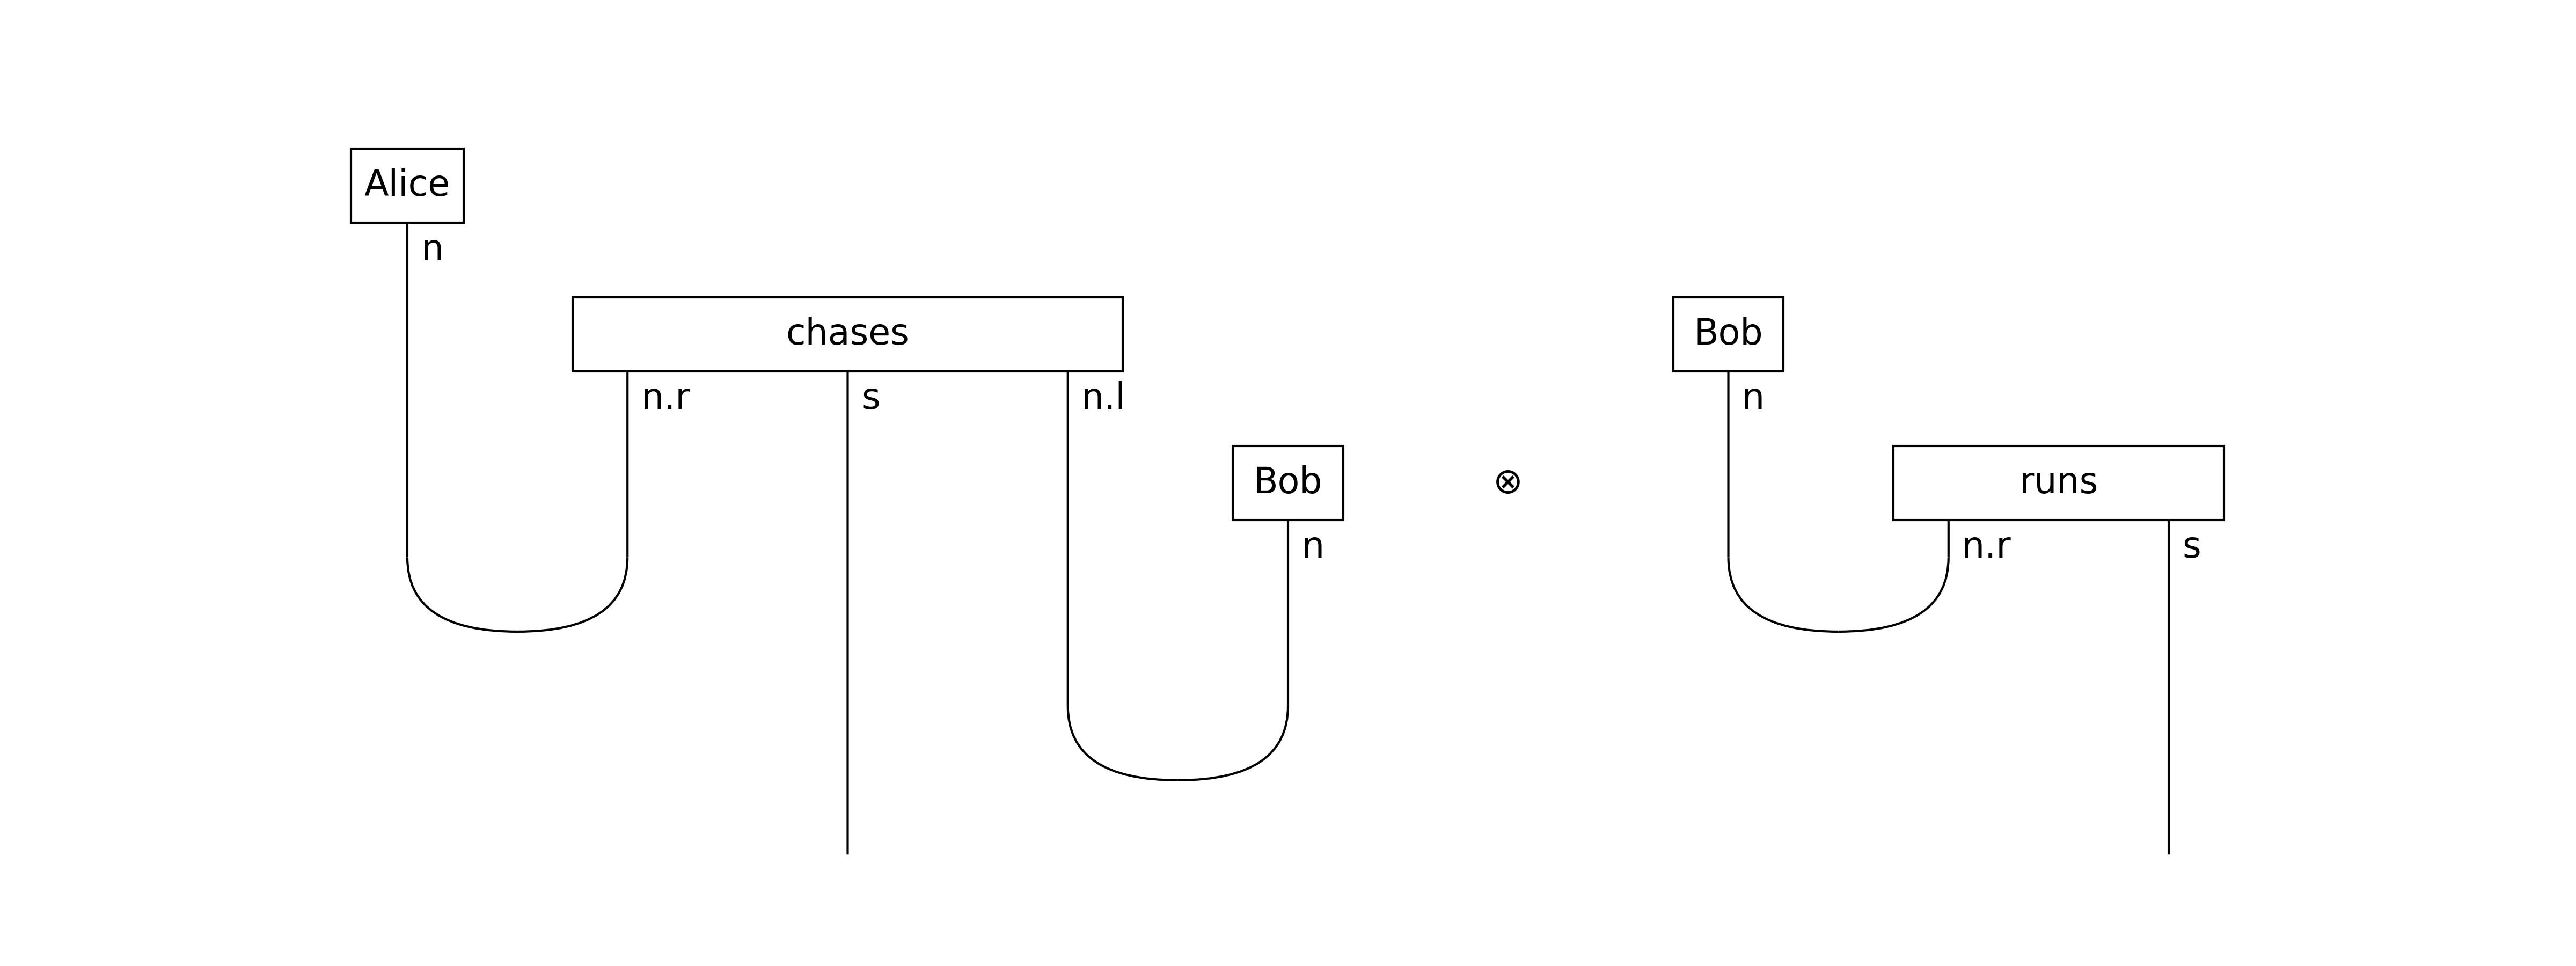
\includegraphics[keepaspectratio,alt={A DisCoCirc-style discourse diagram for the two-sentence discourse ``Alice chases Bob. Bob runs.'' generated via DisCoPy's pregroup grammar. Sentence 1: three Word boxes contract Alice (n) and Bob (n) into the transitive verb ``chases'' (n\^{}r \textbackslash otimes s \textbackslash otimes n\^{}l), producing sentence type s. Sentence 2: Bob (n) contracts into the intransitive ``runs'' (n\^{}r \textbackslash otimes s), producing a second s. The full discourse type is the tensor product s \textbackslash otimes s, encoding inter-sentential coherence through parallel compositional structure. In a full DisCoCirc implementation, the shared entity wire for Bob would carry accumulated semantic state across the sentence boundary---the foundation for case role tracking in .}]{../figures/discopy_discocirc_discourse.png}}
\caption{A DisCoCirc-style discourse diagram for the two-sentence
discourse ``Alice chases Bob. Bob runs.'' generated via DisCoPy's
pregroup grammar. \textbf{Sentence 1}: three Word boxes contract Alice
(\(n\)) and Bob (\(n\)) into the transitive verb ``chases''
(\(n^r \otimes s \otimes n^l\)), producing sentence type \(s\).
\textbf{Sentence 2}: Bob (\(n\)) contracts into the intransitive
``runs'' (\(n^r \otimes s\)), producing a second \(s\). The full
discourse type is the tensor product \(s \otimes s\), encoding
inter-sentential coherence through parallel compositional structure. In
a full DisCoCirc implementation, the shared entity wire for Bob would
carry accumulated semantic state across the sentence boundary---the
foundation for case role tracking in
\autoref{fig:three-sentence-discourse}.}\label{fig:discourse}
\end{figure}
\end{frame}

\begin{frame}{Case Role Reversal Across Discourse Boundaries}
\protect\phantomsection\label{case-role-reversal-across-discourse-boundaries}
The power of DisCoCirc for case theory becomes particularly vivid in
multi-sentence discourses where the \emph{same entity occupies different
case roles} across sentences. Consider the three-sentence discourse:

\begin{quote}
\emph{``Alice chases Bob. Bob fears Alice. She smiles.''}
\end{quote}

In this discourse, Alice undergoes a complete cycle of case role
reversals:

\begin{enumerate}
\tightlist
\item
  \textbf{Sentence 1}: Alice is \(\text{NOM}\) (Proto-Agent, the one
  chasing) and Bob is \(\text{ACC}\) (Proto-Patient, the one chased).
\item
  \textbf{Sentence 2}: Bob is now \(\text{NOM}\) (the one fearing) and
  Alice is \(\text{ACC}\) (the one feared)---a role reversal where Alice
  moves from agent to patient.
\item
  \textbf{Sentence 3}: ``She'' resolves anaphorically to Alice, who
  returns to \(\text{NOM}\) as the agent of smiling.
\end{enumerate}

This NOM → ACC → NOM trajectory for Alice across three sentences is
precisely the kind of \emph{dynamic case assignment} that static
single-sentence analyses cannot capture. The categorical representation
as a triple tensor product \(s \otimes s \otimes s\)
(\autoref{fig:three-sentence-discourse}) encodes each sentence as an
independent pregroup derivation while preserving the entity identity
that links them. In a full DisCoCirc implementation, Alice's entity wire
would carry accumulated semantic state---the meaning of ``She'' in
sentence 3 inherits the enriched state of an Alice who has first chased
and then been feared, not merely the bare lexical entry for ``Alice.''

\begin{figure}
\centering
\pandocbounded{\includegraphics[keepaspectratio,alt={Three-sentence discourse diagram for ``Alice chases Bob. Bob fears Alice. She smiles.'' rendered using DisCoPy, demonstrating dynamic case role reversal. Sentence 1: Alice is NOM (Proto-Agent), Bob is ACC (Proto-Patient). Sentence 2: Bob is NOM, Alice is ACC---a complete agent--patient role reversal. Sentence 3: the anaphoric pronoun ``She'' resolves to Alice, who returns to NOM. Alice's case trajectory NOM\textbackslash toACC\textbackslash toNOM across three sentences is tracked by the triple tensor product s \textbackslash otimes s \textbackslash otimes s. In a full DisCoCirc implementation, Alice's entity wire would carry accumulated semantic state---the meaning of ``She'' in sentence 3 inherits the enriched state of an Alice who has first chased and then been feared, not merely the bare lexical entry for ``Alice.'' This dynamic case assignment across discourse boundaries is precisely what lambeq Gen II {[}@lambeq2025genii{]} can compile into parameterized quantum circuits.}]{output/figures/discopy_three_sentence_discourse.png}}
\caption{Three-sentence discourse diagram for ``Alice chases Bob. Bob
fears Alice. She smiles.'' rendered using DisCoPy, demonstrating dynamic
case role reversal. \textbf{Sentence 1}: Alice is NOM (Proto-Agent), Bob
is ACC (Proto-Patient). \textbf{Sentence 2}: Bob is NOM, Alice is
ACC---a complete agent--patient role reversal. \textbf{Sentence 3}: the
anaphoric pronoun ``She'' resolves to Alice, who returns to NOM. Alice's
case trajectory NOM\(\to\)ACC\(\to\)NOM across three sentences is
tracked by the triple tensor product \(s \otimes s \otimes s\). In a
full DisCoCirc implementation, Alice's entity wire would carry
accumulated semantic state---the meaning of ``She'' in sentence 3
inherits the enriched state of an Alice who has first chased and then
been feared, not merely the bare lexical entry for ``Alice.'' This
dynamic case assignment across discourse boundaries is precisely what
lambeq Gen II {[}@lambeq2025genii{]} can compile into parameterized
quantum circuits.}\label{fig:three-sentence-discourse}
\end{figure}
\end{frame}

\begin{frame}{Quantum NLP and the lambeq Pipeline}
\protect\phantomsection\label{quantum-nlp-and-the-lambeq-pipeline}
The categorical structure of DisCoCat maps naturally onto quantum
circuits: the tensor product structure of \(\mathbf{FVect}\) is
identical to the tensor product structure of \(\mathbf{Qubit}\), the
category of qubit systems. This observation underlies the \textbf{QNLP}
(Quantum Natural Language Processing) program
{[}@meichanetzidis2020qnlp{]}, which implements DisCoCat models as
parameterized quantum circuits.

The \textbf{lambeq} library {[}@lorenz2023lambeq{]} provides a practical
pipeline:

\begin{enumerate}
\tightlist
\item
  Parse a sentence into a pregroup derivation (via the neural CCG parser
  Bobcat or rule-based parsers)
\item
  Convert the derivation into a string diagram
\item
  Translate the diagram into a parameterized quantum circuit (or a
  classical tensor network)
\item
  Train the parameters on NLP tasks (classification, similarity,
  question answering)
\end{enumerate}

Kartsaklis et al. {[}-@kartsaklis2021functorial{]} demonstrate that this
pipeline achieves competitive performance on question-answering tasks,
confirming that the categorical structure captures genuine linguistic
regularities even when instantiated on noisy near-term quantum hardware.

\textbf{lambeq Gen II} (released May 2025) marks a significant advance
by incorporating full \textbf{DisCoCirc} support as its core
mathematical foundation, enabling the framework to scale beyond
single-sentence semantics to discourse-level NLP {[}@lambeq2025genii{]}.
With over 50,000 downloads, lambeq Gen II achieves language neutrality,
improved trainability, and compositional interpretability for
explainable AI on quantum hardware. DisCoCirc's state wires---which
track entity persistence across sentence boundaries---can now be
automatically compiled into parameterized quantum circuits, closing the
gap between sentence-level DisCoCat and discourse-level case role
tracking. This is directly relevant to the case role reversal phenomena
discussed in \autoref{fig:three-sentence-discourse}: lambeq Gen II can,
in principle, compile such multi-sentence case-dynamic discourses into
trainable quantum circuits.

Recent work on quantum-cognitive frameworks integrates DisCoCat and
DisCoCirc with density matrices for modeling dynamic meaning in text,
treating semantic states as mixed quantum states that evolve through
discourse---providing an alternative to pure-state vector models that
naturally accommodates ambiguity and partial information
{[}-@quantumcognitive2026frontiers{]}.

Recent work on \textbf{string diagram rewriting} by Bonchi et al.
{[}-@bonchi2022rewriting{]} provides the theoretical foundation for
diagram simplification, showing that string diagram rewrite systems
modulo Frobenius structure can be interpreted as double-pushout
hypergraph rewriting---ensuring that the algebraic simplifications
applied during normal form computation are provably sound. De Huybrecht
{[}-@dehuybrecht2024subcategorizing{]} extends DisCoCat with
\emph{subcategorization} for light verb constructions, demonstrating
that the categorical framework accommodates sublexical compositional
structure---a development that connects naturally to the monadic root
syntax of Song {[}-@song2022act{]} discussed in
\autoref{sec:categorial-grammar}.

For our case-theoretic framework, QNLP offers a concrete computational
substrate: case categories could be implemented as quantum circuits
where case roles correspond to quantum registers and grammatical
relations correspond to parameterized gates. This connection between
linguistic case structure and quantum information processing---mediated
entirely by the shared categorical formalism---illustrates the power of
the diagrammatic approach.

\newpage
\end{frame}

\end{document}
